\begin{frame}
\frametitle{FEniCS has been used for a wide range of
  equations and applications}

{\tiny Reaction-diffusion equations; Stokes with or without nonlinear
  viscosity; compressible and incompressible Navier--Stokes; RANS
  turbulence models; shallow water equations; Bidomain equations;
  nonlinear and linear elasticity; nonlinear and linear
  viscoelasticity; Schr\"odinger; Biot's equations for porous media,
  fracture mechanics, electromagnetism, liquid crystals including
  liquid crystal elastomers, combustion, ... and coupled systems of
  the above, ...}

\begin{center}
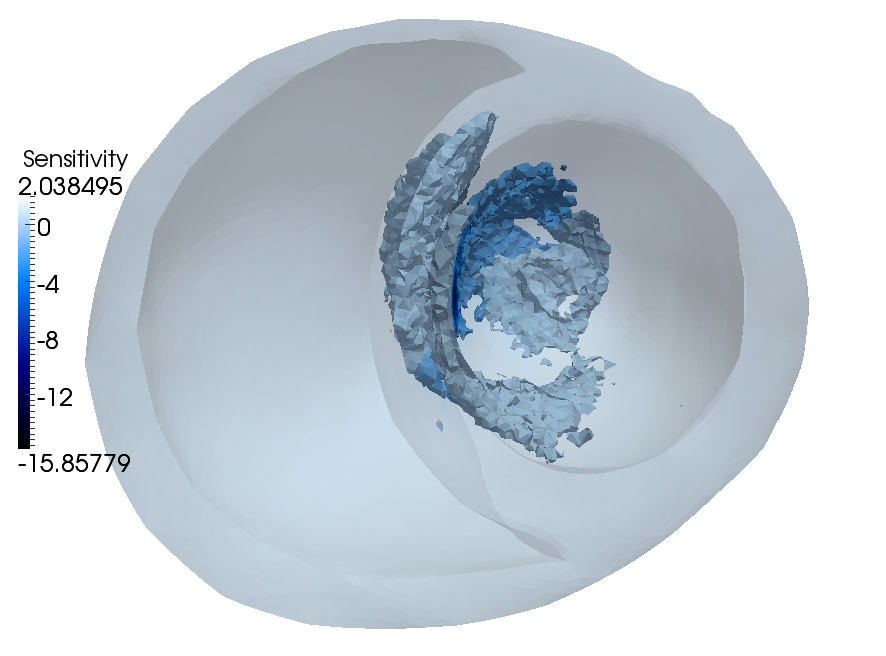
\includegraphics[width=0.24\textwidth]{png/g_el_plusx.png}
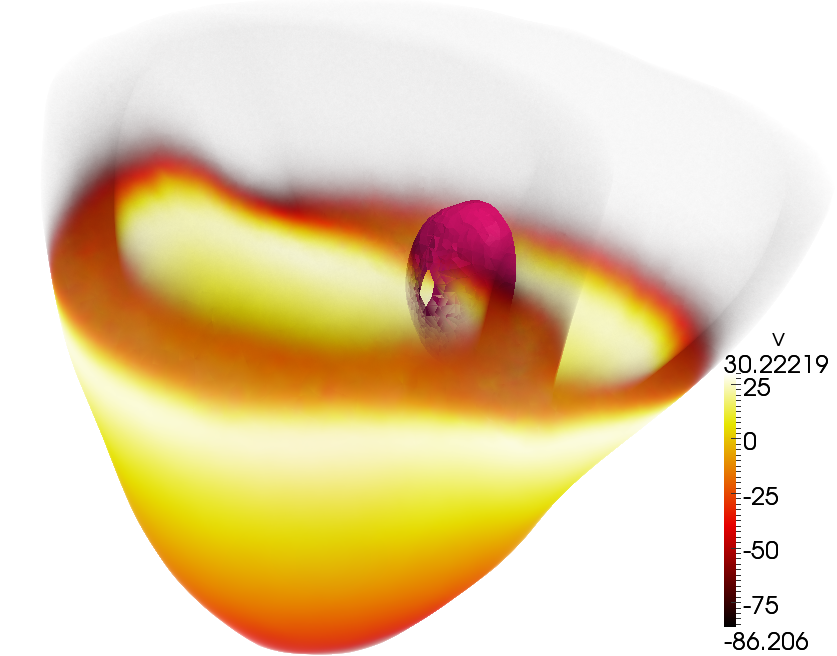
\includegraphics[width=0.24\textwidth]{png/unhealthy_v_at_T200.png}
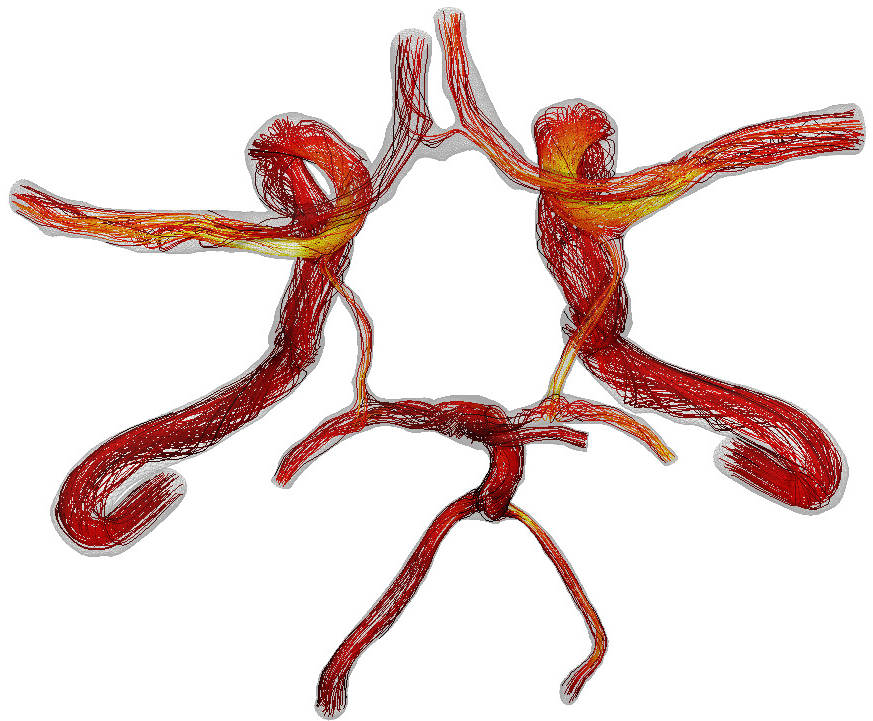
\includegraphics[width=0.24\textwidth]{png/circle_of_willis_simulation.png}
\end{center}

{\tiny for simulating blood flow, computing calcium release in cardic
  tissue, computing the cardiac potential in the heart, simulating
  mantle convection, simulating melting ice sheets, computing the
  optimal placement of tidal turbines, simulating and reconstructing
  tsunamis, simulating the flow of cerebrospinal fluid and the
  deformation of the spinal cord, simulating waveguides, ... }

\end{frame}
